\section{Results} \label{sec:evals}

Our algorithm is implemented in the aligner
\astarpa%
\footnote{\href{https://github.com/RagnarGrootKoerkamp/astar-pairwise-aligner}{github.com/RagnarGrootKoerkamp/astar-pairwise-aligner}
(\href{https://github.com/RagnarGrootKoerkamp/astar-pairwise-aligner/tree/1e3841e239093fc32ccc2eb3af1d2fe0da240b6e}{1e3841e})}
in Rust. We compare it with state of the art exact aligners on
synthetic~(\cref{GLOBALsec:evals-comparison-synthetic}) and
human~(\cref{GLOBALsec:evals-comparison-hg})
data%
\footnote{\href{https://github.com/pairwise-alignment/pa-bench/releases/tag/datasets}{github.com/pairwise-alignment/pa-bench/releases/tag/datasets}}
using \pabench%
\footnote{\href{https://github.com/pairwise-alignment/pa-bench}{github.com/pairwise-alignment/pa-bench}
(commit
\href{https://github.com/pairwise-alignment/pa-bench/commit/55db71002d6a0ef5623a231a8c19085e34712223}{55db710})}%
.
We justify our heuristics and optimizations by comparing their scaling and
performance~(\cref{sec:techniques}).

\begin{figure*}[H]
    %\vspace{-1.66em}
    \centering
    \hfill
    \subfloat[Runtime scaling with length ($d{=}4\%$, $r{=}1$)]
    {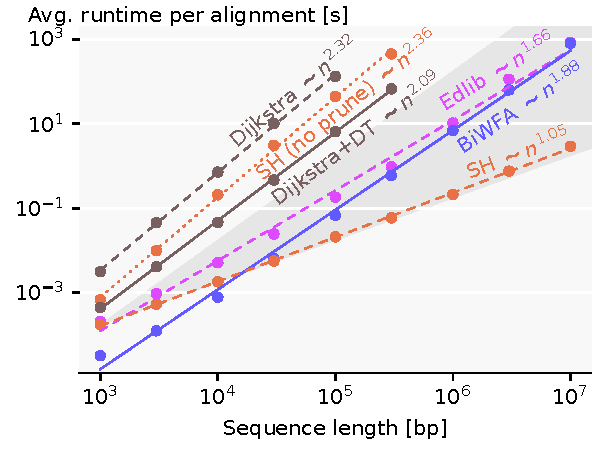
\includegraphics[scale=0.55]{plots/scaling_n.labels.pdf}\label{fig:scaling-n}}
    \hfill
    \subfloat[Runtime scaling with length ($d{=}12\%$, $r{=}2$)\!\!]
    {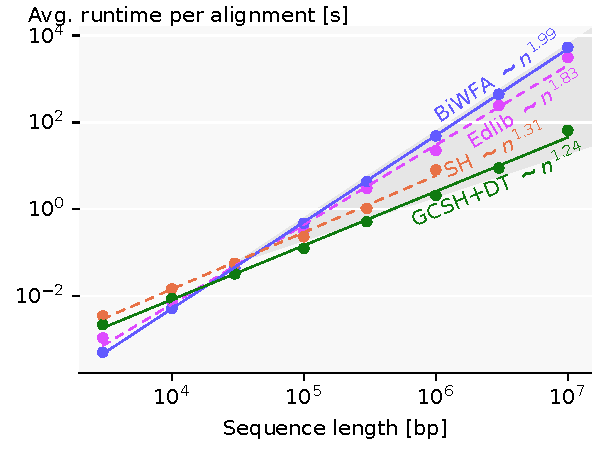
\includegraphics[scale=0.55]{plots/tools_e0.15_enlarged.labels.pdf}\label{fig:scaling-n-large}}
    \hfill
    \subfloat[Runtime scaling with divergence]
    {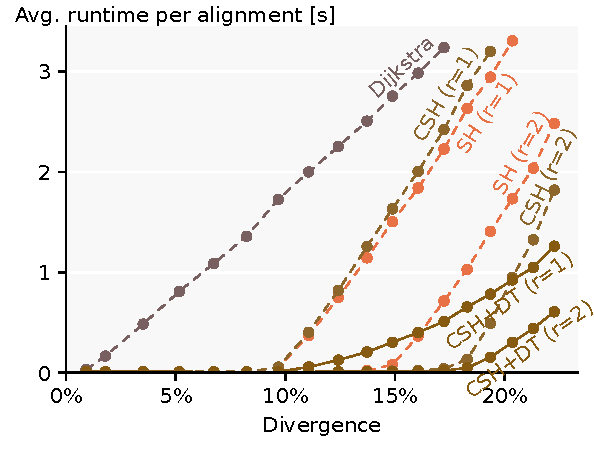
\includegraphics[scale=0.55]{plots/scaling_e.labels.pdf}\label{fig:scaling-e}}
    \hfill
    \caption[Runtime scaling on synthetic data]{
      \textbf{Runtime comparison on synthetic data}
      \protect\subref{fig:scaling-n}\protect\subref{fig:scaling-n-large}
  Log-log plots comparing our simplest~(\SH) and most accurate
  heuristic~(\GCH with DT) to \edlib, \wfa, and other algorithms
      (averaged over $10^6$ to $10^7$ total bp, seed length $k{=}15$).
  The slopes of the bottom (top) of the dark-grey cones correspond to linear (quadratic) growth.
      \SH without
      pruning is dotted, and variants with DT are solid. At $4\%$ divergence,
      the complex techniques \CSH, \GCH, and DT (not shown) are as fast as \SH.
  Missing data points are due to exceeding the $\qty{32}{GiB}$ memory limit.
  \protect\subref{fig:scaling-e}
  Runtime scaling with divergence ($n{=}10^4$, $10^6$ total bp, $k{=}10$).
      \GCH (not shown) is as fast as \CSH.}
    \label{fig:synthetic}
\end{figure*}

\subsection{Setup} \label{sec:evals-setup}

\paragraph{Synthetic data}
Our synthetic datasets are parameterized by sequence length~$n$, induced error
rate~$e$, and total number of basepairs~$N$, resulting in $N/n$ sequence pairs.
The first sequence in each pair is uniform-random from~$\Sigma^n$. The second is
generated by sequentially applying~$\lfloor e{\cdot} n\rfloor$ edit operations
(insertions, deletions, and substitutions with equal~$1/3$ probability) to the
first sequence. Introduced errors can cancel each other, making the
\emph{divergence}~$d$ between the sequences less than~$e$. Induced error rates
of $1\%$, $5\%$, $10\%$, and~$15\%$ correspond to divergences of $0.9\%$,
$4.3\%$, $8.2\%$, and~$11.7\%$, which we refer to as $1\%$, $4\%$, $8\%$,
and~$12\%$.

\paragraph{Human data}
We use two datasets%
of ultra-long Oxford Nanopore Technologies (ONT) reads of the human genome: one
without and one with genetic variation. All reads are $500\mbox{--}1100\kbp$
long, with mean divergence around $7\%$. The average length of the longest gap
in the alignment is
$0.1\kbp$ for ONT reads, and $2\kbp$ for ONT reads with genetic
variation~(detailed statistics in~\cref{tab:hg}).
The reference genome is
CHM13~(v1.1)~\citep{nurk2022complete}. The reads used for each dataset are:

\begin{itemize}
  \item \emph{ONT}: $50$ reads sampled from those used to assemble
        CHM13.
  \item \emph{ONT with genetic variation}: $48$~reads from another
        human~\citep{bowden2019sequencing}, as used in the \wfa
        paper~\citep{marco2022optimal}.
\end{itemize}

\paragraph{Algorithms and aligners}
We compare \SH, \CSH, and \GCH as implemented in \astarpa%
to the state-of-the-art exact aligners \wfa and \edlib. We also compare to
\dijkstra and to variants without pruning, and without diagonal transition. We
exclude \seqan and \parasail since they are outperformed by \wfa and
\edlib~\citep{marco2021fast}.

\paragraph{\astarpa parameters}
We run all aligners with unit edit costs with traceback enabled, returning an
alignment. In \astarpa we fix $r{=}2$ (inexact matches) and seed length
$k{=}15$. Both are a trade-off: inexact matches and lower $k$ increase the
heuristic potential to efficiently handle more divergent sequences, while too
low $k$ gives too many matches.

\paragraph{Execution}
We use
\pabench
on Arch Linux on an \texttt{Intel Core i7-10750H} processor with $\qty{64}{GB}$
of memory and $6$ cores, without hyper-threading, frequency boost, and CPU power saving
features. We fix the CPU frequency to \texttt{2.6GHz}, limit the memory usage to
$\qty{32}{GiB}$, and run $1$ single-threaded job at a time with niceness $-20$.

\paragraph{Measurements}
\pabench first reads the dataset from disk and then measures the wall-clock time
and increase in memory usage of each aligner. Plots and tables refer to the
average alignment time per aligned pair. Best-fit polynomials are calculated via
a linear fit in the log-log domain using the least squares method.


\begin{figure}[H]
  \centering
  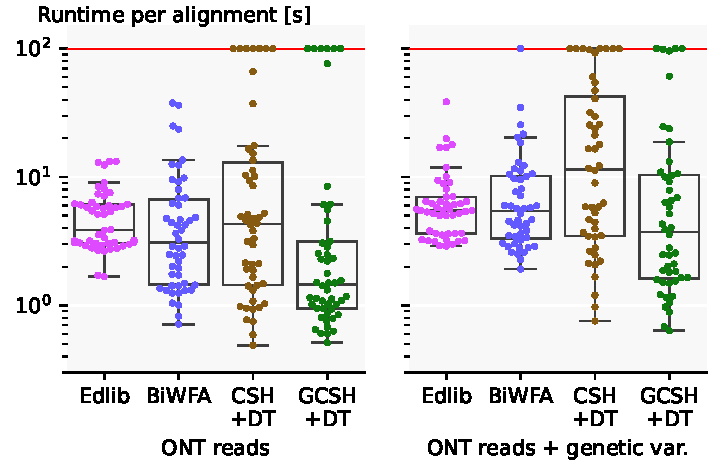
\includegraphics[scale=0.50]{plots/real_summary.pdf}
  \caption[Runtime of \astarpa on long human reads]{\textbf{Runtime on long
      human reads.} Each dot is an alignment without (left) and with (right)
      genetic variation. Runtime is capped at $\qty{100}{s}$. The median speedup
      of \astarpa~(\GCH + DT, $k{=}15$, $r{=}2$) is $2\times$~(left) and
      $1.4\times$~(right) over \edlib and \wfa.}
  \label{fig:human-summary}
\end{figure}

\subsection{Comparison on synthetic data} \label{GLOBALsec:evals-comparison-synthetic}

Here we compare the runtime scaling and performance of the exact optimal
aligners on synthetic data.
\cref{GLOBALsec:techniques} compares the effects of pruning and inexact matches,
whereas~\cref{GLOBALsec:expanded} compares \SH and \CSH in terms of the number of
expanded states.

\paragraph{Scaling with sequence length}
% figs: better scaling => faster for long
First, we compare the aligners by runtime scaling with sequence length $n$ for
various error rates $e$ (\cref{GLOBALfig:scaling-n}). As expected from the theoretical
analysis, \edlib and \wfa scale approximately quadratically regardless of the
error rate. Unlike them, \SH and \CSH scale subquadratically which explains why
they are faster for long enough sequences.

% for low error rates
More specifically, for low error rates ($e{=}1\%$ and $e{=}5\%$), both \SH and
\CSH with exact matches scale near-linearly with sequence length (best
fit~$n^{1.08}$ for \mbox{$n{\le}10^7$}), and the benefit from chaining is
negligible.

% for high error rates
For high error rates ($e{\geq}10\%$) and large $n$, the need to match the seeds
inexactly causes a significant number of off-path matches. These off-path
matches lower the value of the heuristics and prevent the punishment of
suboptimal paths. This causes \SH to expand a super-linear number of states
(\cref{GLOBALsec:expanded}). Chaining the matches enforces them
to follow the order of the seeds, which greatly reduces the negative effects of
the off-path matches, leading to only linearly many expanded states.
Nevertheless, the runtime scaling of \CSH
is super-linear as a result of the increasing fraction of time (up to $93\%$ for
$n{=}10^7$) spent on reordering states because of outdated $f$ values after
pruning.

%(TODO: high variance; more seqs needed)
\paragraph{Performance}
\cref{GLOBALtab:evals} compares the runtime and memory of \astarpa with match
pruning to \edlib (based on banding, exponential search, bit-parallel) and \wfa
(based on diagonal transition and divide \& conquer) for aligning a single pair
of sequences of length $n{=}10^7$. \A with \CSH (\cshsymbol~\cshsymbolsq) is
more than $250$ times faster than \edlib and \wfa at $e{=}5\%$. For low error
rate ($e{\leq}5\%$), there is no significant performance difference between \SH
(\shsymbol~\shsymbolsq) and \CSH. The memory usage of \astarpa for $e{\leq}5\%$
is less than $\qty{600}{MB}$ for any $n$. At $e{=}15\%$, \CSH uses at most
$\qty{4.7}{GB}$ while \SH goes out of memory ($\geq\qty{30}{GB}$) because there
are too many expanded states to store.

   
%& \A, match-pruning, \sh                      
%& \A, match-pruning, \csh                     

\subsection{Comparison on real data} \label{GLOBALsec:evals-comparison-hg}

\begin{figure}[H]
  \centering
  \subfloat[CHM13: ONT read errors]%
  {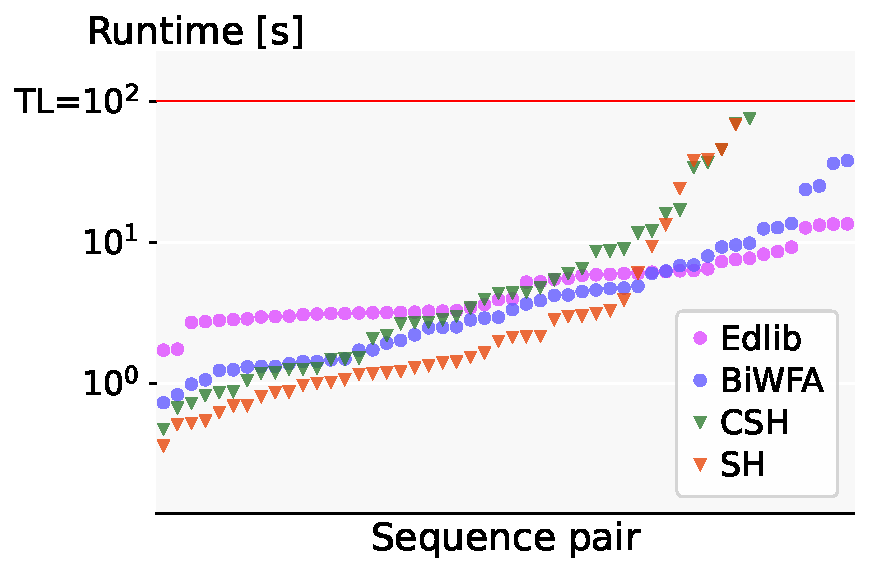
\includegraphics[width=0.48\linewidth]{imgs/fig7/human_sorted_chm13.pdf}}
  \hfill
  \subfloat[NA12878: ONT read errors + biological variation]%
  {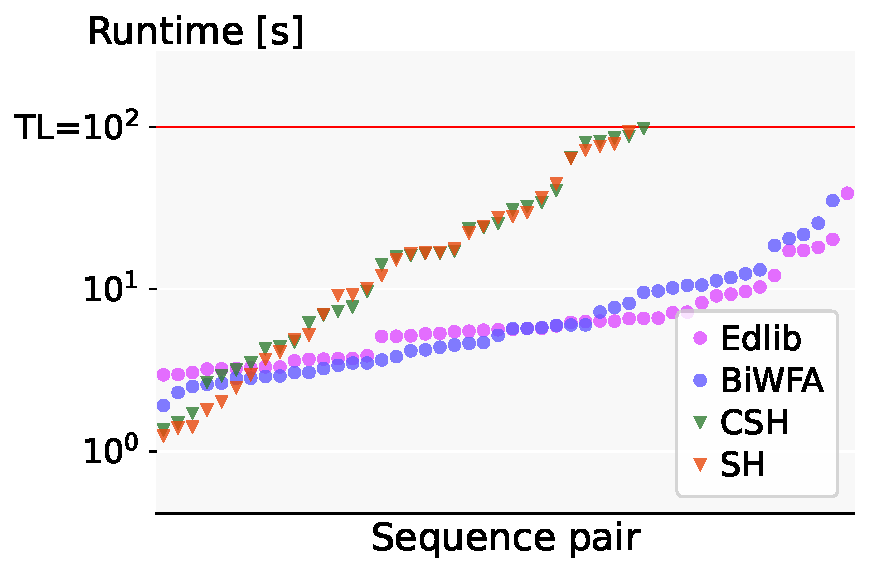
\includegraphics[width=0.48\linewidth]{imgs/fig7/human_sorted_na12878.pdf}}
  \caption[Runtime per sequence (real data)]{Log plot comparison of the
  aligners' runtime on \textbf{real data}. The data points for each individual
  aligner are sorted by alignment time. Alignments that timed out after $100$
  seconds are not shown.}
  \label{GLOBALfig:human-results}
\end{figure}

In this section we compare the exact optimal aligners on long ONT reads from our
human datasets~(\cref{GLOBALfig:human-results}). With the presented minimalistic
features, \astarpa aligns some sequences faster than \wfa and \edlib, but the
high runtime variance makes it slower overall~(\cref{GLOBALsec:variation-human-results}).

% heuristics vs biwfa/edlib
On the dataset without biological variation \datasetOne, \SH is faster than \wfa
and \edlib on $58\%$ of the alignments ($29$ of $50$). On the dataset with
biological variation \datasetTwo, \SH outperforms \wfa and \edlib on $17\%$ of the
alignments ($8$ of $48$) and in other cases is over an order of magnitude
slower. In both datasets, \SH and \CSH time out for the sequences with the
highest edit distances, because they have an error rate larger than the
heuristic can handle efficiently~($e\geq r/k=2/15=13.3\%$).

% SH vs CSH
\CSH usually explores fewer states than \SH since \csh dominates
the \sh. However, in certain cases \CSH is slower than \SH since needs more time
to update the heuristic after pruning (Step 3$'$ in \cref{GLOBALsec:compute-csh}).
%, and %spends up to $98\%$ of its time on this.

\subsection{Effect of pruning, inexact matches, chaining, and DT}\label{sec:techniques}

We visualize the effects of complex sequences on the \A
search~(\cref{app:comparison}).

\paragraph{Pruning enables near-linear runtime}
\Cref{fig:scaling-n} shows that match pruning changes the quadratic runtime of
\SH to near-linear, by penalizing the expansion of states before the search tip.

\paragraph{Inexact matches cope with higher divergence}
Inexact matches increase the heuristic potential, allowing higher
divergence~(\cref{fig:scaling-e}). For low divergence, the runtime is nearly
constant~(\cref{app:scaling-e}), while for higher divergence it switches to
linear. Inexact matches nearly double the threshold for constant runtime from
$d\leq10\% = 1/k$ to $d\leq18\% \approx2/k$.

\paragraph{Chaining copes with spurious matches}
When seeds have many spurious matches (typical for inexact
matches, $r{=}2$ in~\cref{fig:scaling-e}), \SH loses its strength. \CSH reduces the
degradation of \SH by chaining matches.

\paragraph{Gap-chaining copes with indels}
Gap costs penalize both short and long indels which are common in genetic
variation. As a result, \GCH is significantly faster than \CSH with genetic
variation~(\cref{fig:human-summary}).

\paragraph{Diagonal transition speeds up quadratic search}
When \A explores quadratically many states, it behaves similar to \dijkstra. DT
speeds up \dijkstra $20\times$~(\cref{fig:scaling-n}) and \CSH
$3\times$~(\cref{fig:scaling-e}). For \dijkstra this is close to $1/d$, the
expected reduction in number of expanded states. DT also speeds up the alignment
of human data~(\cref{app:human}).

